\documentclass[12pt]{article}
        \usepackage{graphicx,type1cm,eso-pic,color}
        \usepackage{hyperref}
        \usepackage[left=3.0cm,right=3.0cm,top=2cm,bottom=2cm,headheight=13.6pt]{geometry}
        \usepackage{subfigure}

\makeatother


\title{Manual for HPS ECal v1.7}

\author{ECal On-Call Cell Phone: 757-810-1489 \\ 
Authors: \\
General contact: Rapha\"el \textsc{Dupr\'e} (\texttt{dupre@ipno.in2p3.fr})\\ 
LED system: Andrea \textsc{Celentano} (\texttt{andrea.celentano@ge.infn.it})\\
LV/HV supply and chiller: Nathan \textsc{Baltzell} (\texttt{baltzell@jlab.org})\\
}

\date{\today} %01/07/2014

\begin{document}
\maketitle{}

   \section{General description of the ECal}


The electromagnetic calorimeter (ECal), installed downstream of the pair spectrometer dipole magnet (figure~\ref{GView}), performs two essential functions for the experiment: it provides the trigger signal and helps identify electrons and positrons. The ECal modules are based on tapered 160 mm long PbWO crystal with a 13.3x13.3 mm$^2$ (16x16 mm$^2$) front (rear) face wrapped in VM2000 multilayer polymer mirror film. The scintillation light, approximately 110 photons / MeV, is read out by a 10x10 mm$^2$ Hamamatsu S8664-1010 Avalanche Photodiode (APD) with 75\% quantum efficiency glued to the rear face surface. The low gain of APDs (150 pC/pC) is compensated with custom-made preamplifier boards, which provide a factor of 225 amplification of the APD signal. In front of the crystals, LEDs are installed to send light into the crystals. These are used in order to check the proper functioning of the ECal and provides complementary information to evaluate gain variations in the various channels of the calorimeter (see figure~\ref{AmplChain}).

\begin{figure}[hp]
\center
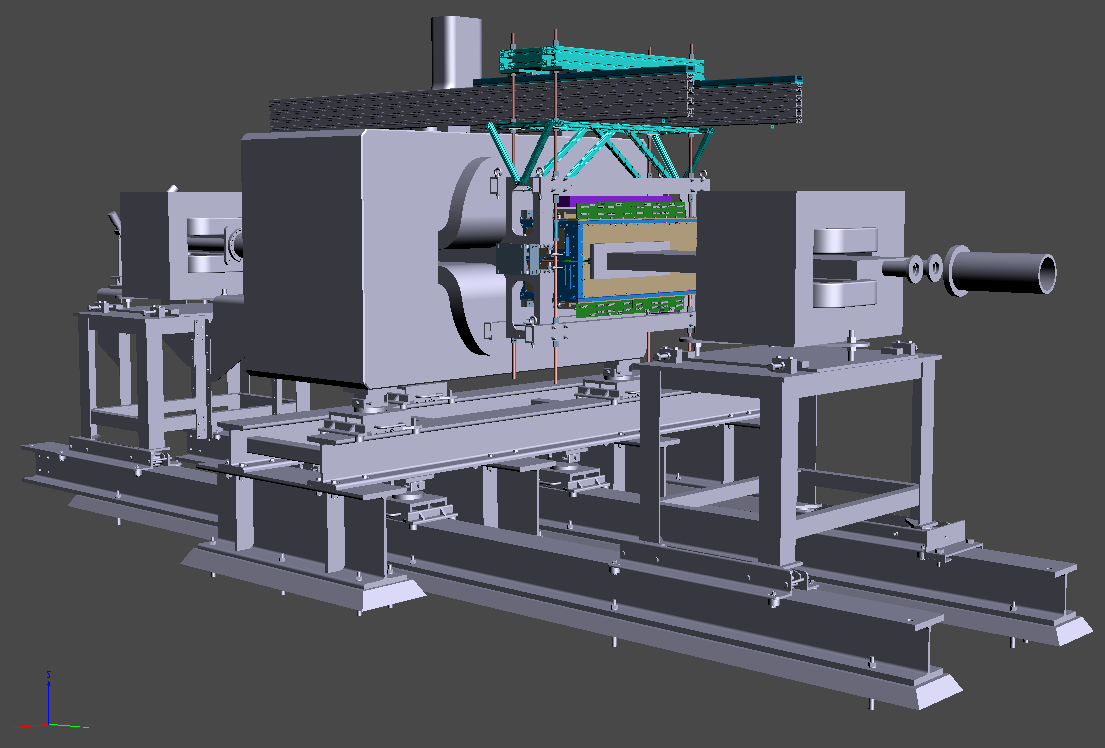
\includegraphics[width=0.75\textwidth]{pics/GView.png}
\caption{\small \label{GView} General view of the ECal (in color) suspended at the downstream end of the HPS analyzing magnet.}
\end{figure}

\begin{figure}[hp]
\center
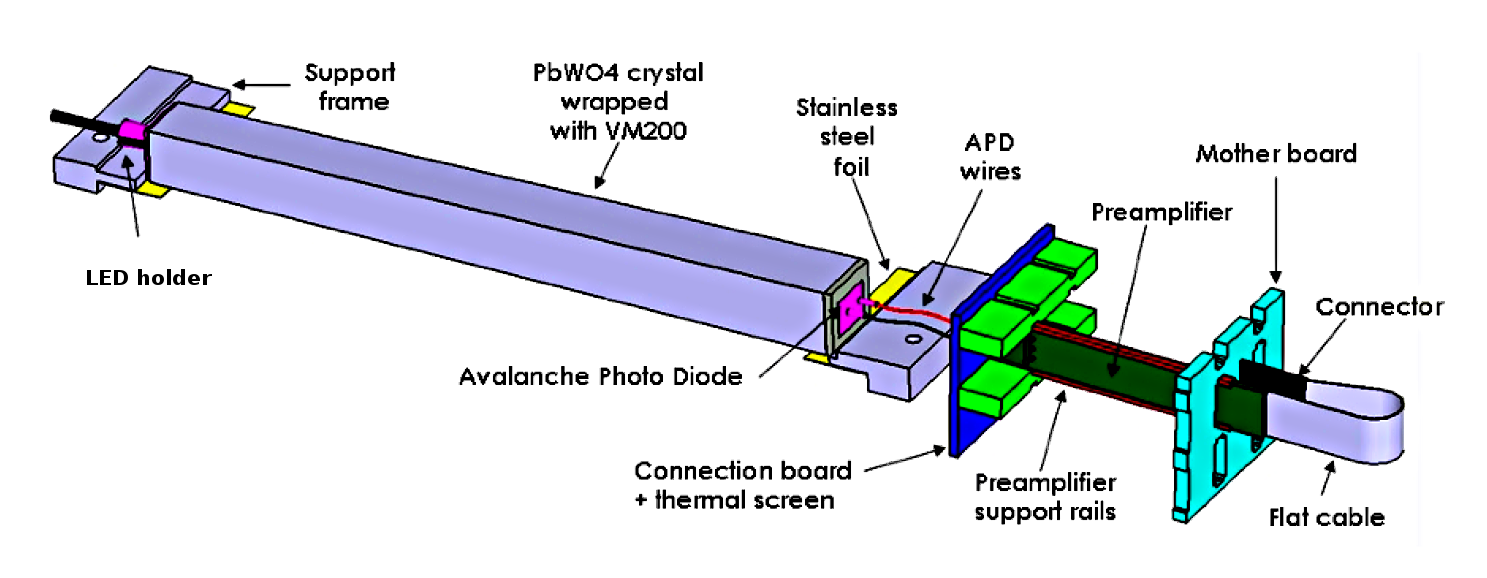
\includegraphics[width=0.75\textwidth]{pics/CrystalAssembly.png}
\caption{\small \label{AmplChain} View of an ECal crystal and the amplification chain.}
\end{figure}
      

\begin{figure}[hp]
\center
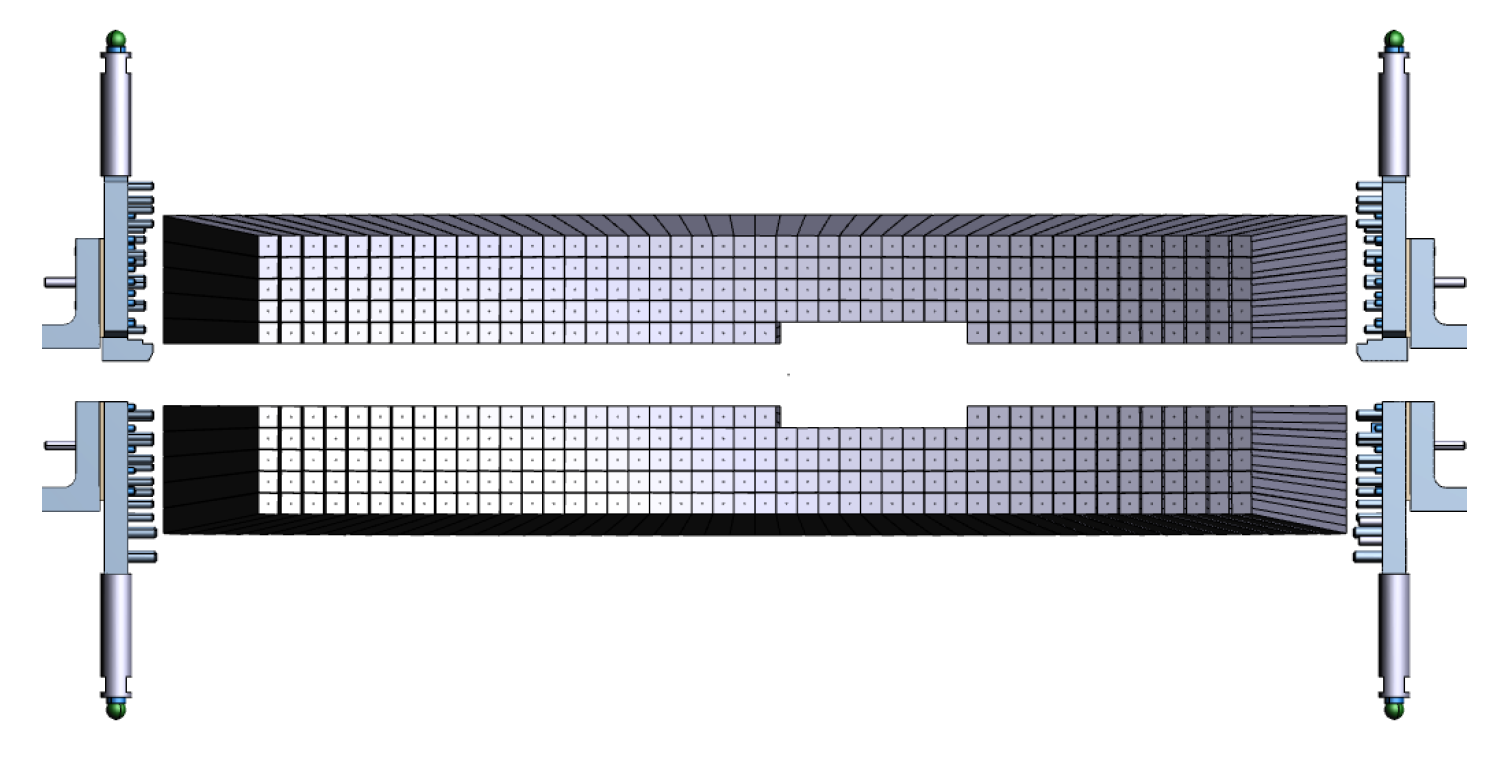
\includegraphics[width=0.75\textwidth]{pics/ECal2.png}
\caption{\small \label{Crystals} Front view of the ECal crystals layout.}
\end{figure}
      
The ECal is built in two separate halves that are mirror reflections of one another relatively to the horizontal plane. The 221 modules in each half are supported by aluminum frames and arranged in rectangular formation with five layers and 46 crystals / layer, except for the layer closest to the beam where nine modules were removed to allow a larger opening for the outgoing electron and photon beams (figure~\ref{Crystals}). Each half is enclosed in a temperature controlled box ( $< 1^\circ$F stability and $< 4^\circ$F uniformity) to stabilize the crystal light yield and the operation of the APDs. Four printed circuit boards (referred as mother boards) mounted on the back plane penetrate the enclosure and are used to supply the $\pm5$ V operating voltage for the preamplifiers, the 400 V bias voltage to the APDs, and to read out signals from the APDs. Each half of the ECal is divided into 26 bias voltage groups formed in order to minimize the gain spread of the APD-preamplifier couples.


After a 2:1 signal splitter, 1/3 of an amplified APD signal is fed to a single channel of a JLab flash ADC (FADC) board. 2/3 of the signal is sent to a discriminator module before a TDC for a time measurement. The FADC boards are high speed VXS modules digitizing up to 16 crystal signals at 250 MHz and storing 4 ns samples with 12-bit resolution. When a trigger is received, the pipeline is read on these boards from 5 samples before and 30 after the trigger time (those values will be adapted during commissioning).

\newpage
 \twocolumn
\part{Shift Takers Instructions}

\vspace*{\stretch{1}}      
Most ECal controls are accessible through EPICS, from the main window (figure~\ref{EPICSmain}). From there you can access {\bf Temperature monitoring} in {\it Miscellaneous} then {\it ECal Temperature}, the {\bf ECal chiller} in {\it Devices} then {\it Chiller (ECAL)}, the {\bf Scalers} in {\it ECal Scaler GUI}, the {\bf ECal high voltage} in {\it Voltages} then {\it ECal HV} and the {\bf LED control panel} in {\it Devices} then {\it Flasher}.  

If not already open, HPS's main EPICS window is opened as user \texttt{hpsrun} on \texttt{clonsl1}, \texttt{clonsl2}, or \texttt{clonsl3}, with the command \begin{center}\texttt{hps\_epics}\end{center}

    {\em   In general, all shift workers should be using user \texttt{hpsrun} for instructions in this document.}
\vspace*{\stretch{1}}      

\begin{figure}[h!]
\center
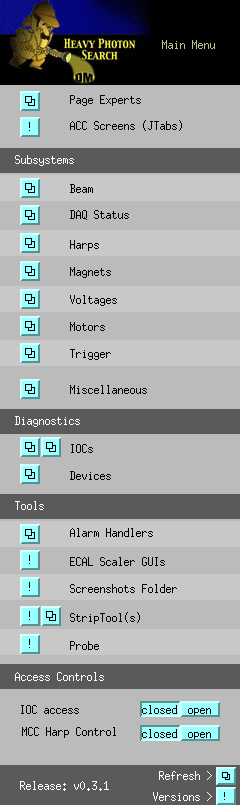
\includegraphics[width=0.38\textwidth]{pics/hps_epics_2014_12_15.png}
\caption{\small \label{EPICSmain} View of the Hall-B EPICS main window.}
\end{figure}

 \onecolumn

      \section{Temperature}

         The ECal temperature should remain as stable as possible in order to avoid gain variation in the system. Eighteen temperature sensors are placed in the ECal enclosure and should be monitored through EPICS (see figure~\ref{temp} and~\ref{temp2}). Variations of two degrees F or more during a shift should be reported to ECal expert on call and noted in the log book.

\begin{figure}[htbp]
\center
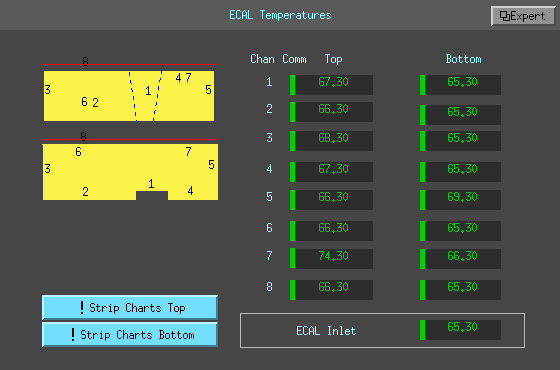
\includegraphics[width=0.5\textwidth]{pics/EcalTemp_2014_12_20.png}
\caption{\small \label{temp} View of the EPICS temperature monitoring window.}
\end{figure}
      
\begin{figure}[htbp]
\center
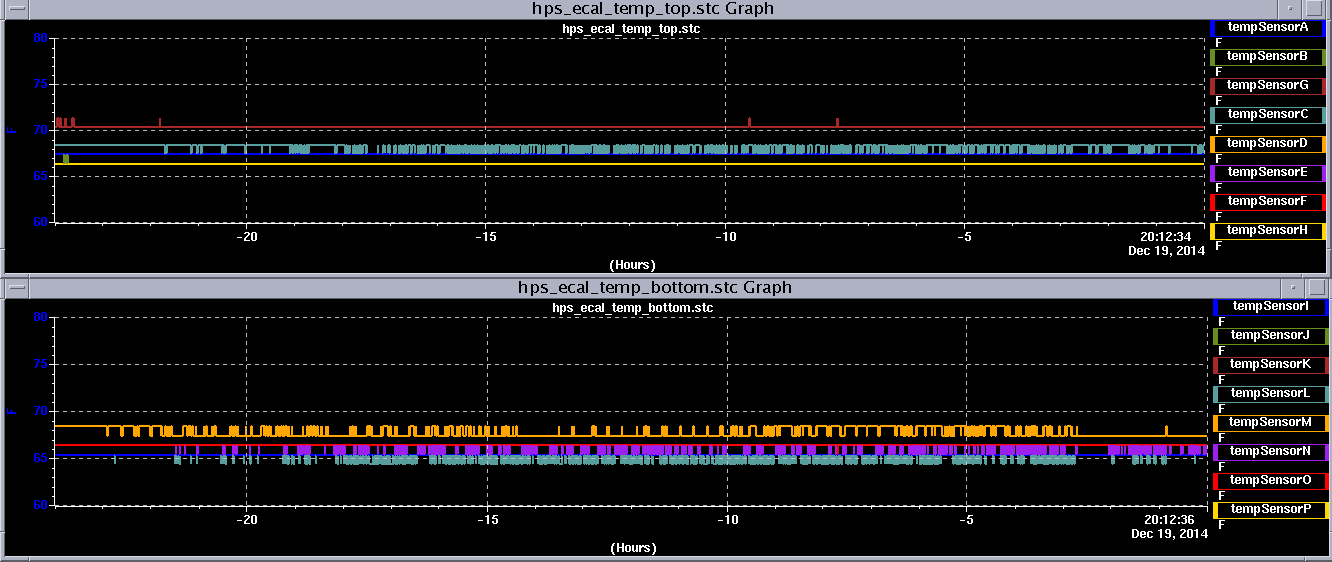
\includegraphics[width=0.8\textwidth]{pics/ECal_temp_s.png}
\caption{\small \label{temp2} View of the EPICS temperature monitoring strip charts.}
\end{figure}

       \section{Chiller}

         The chiller allows to keep the calorimeter at the right temperature and should be ON and set at 17C at all times. The chiller can be monitored through its webcam (figure~\ref{ChillerCam}) or using its EPICS controls (figure~\ref{ChillerCam}). Shift takers should not attempt to change the chiller settings and call ECal expert in case of problem.

         The webcam is accessible either by the url \texttt{cctv10.jlab.org} in a web browser, or via the ``Monitoring'' tab on the main {\bf HPS Run Wiki}.

\begin{figure}[h]
\center
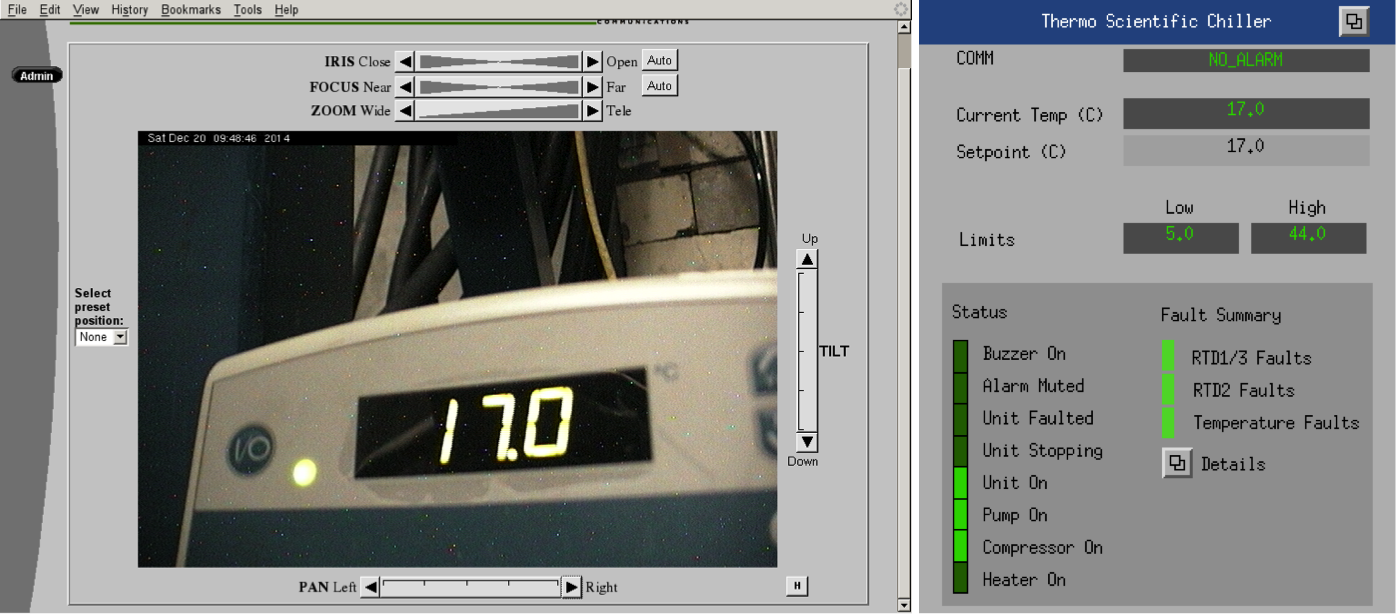
\includegraphics[width=0.99\textwidth]{pics/ChillerCombo.png}
%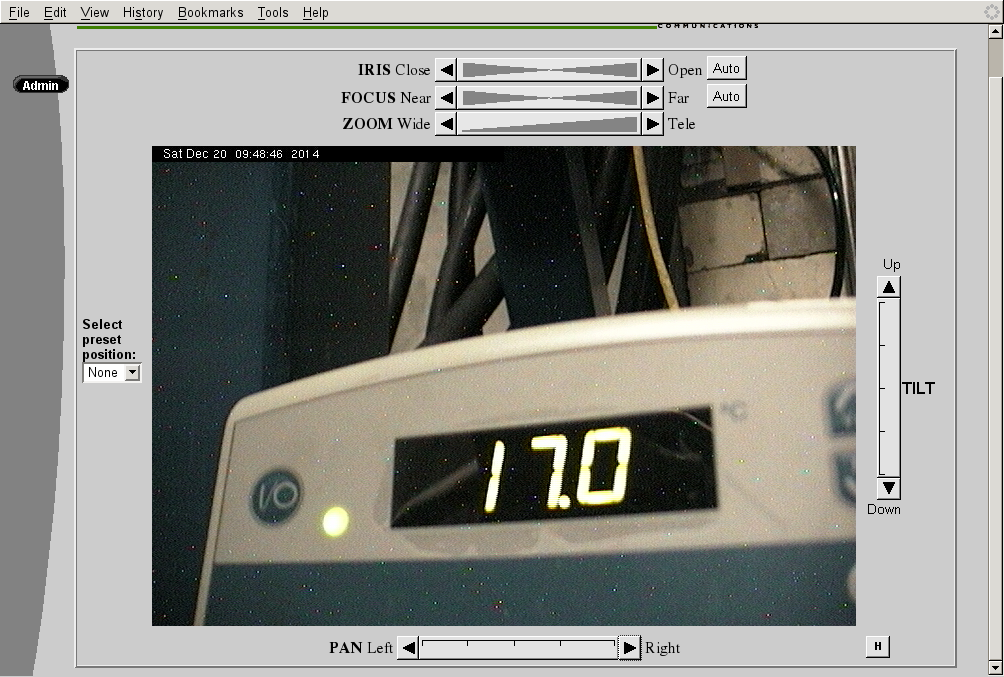
\includegraphics[width=0.5\textwidth]{pics/ChillerCam_2014_12_20.png}
%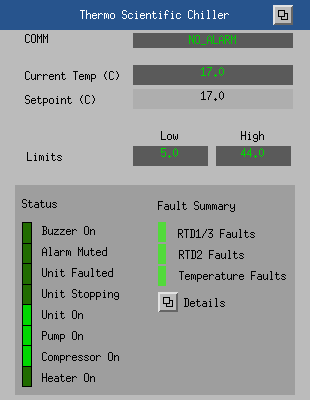
\includegraphics[width=0.45\textwidth]{pics/ChillerWin_2014_12_20.png}
\caption{\small \label{ChillerCam} View of the chiller by webcam (\texttt{cctv10.jlab.org}) and its EPICS window in normal operation.}
\end{figure}



   \section{Voltages}

      \subsection{Low Voltage Controls}

      The low voltage power supply must be on before HV is turned on.  The LV supply is controlled manually in the hall and should be monitored using its webcam (figures~\ref{LVCam}). Call the ECal expert if this appears not to be ON or shows an abnormal current.  Normal current is between 4.0 and 4.2 A.

         A webcam is focused on the LV supply, accessible either by the url \texttt{cctv11.jlab.org} in a web browser, or via the ``Monitoring'' tab on the main {\bf HPS Run Wiki}.

\begin{figure}[htbp]
\center
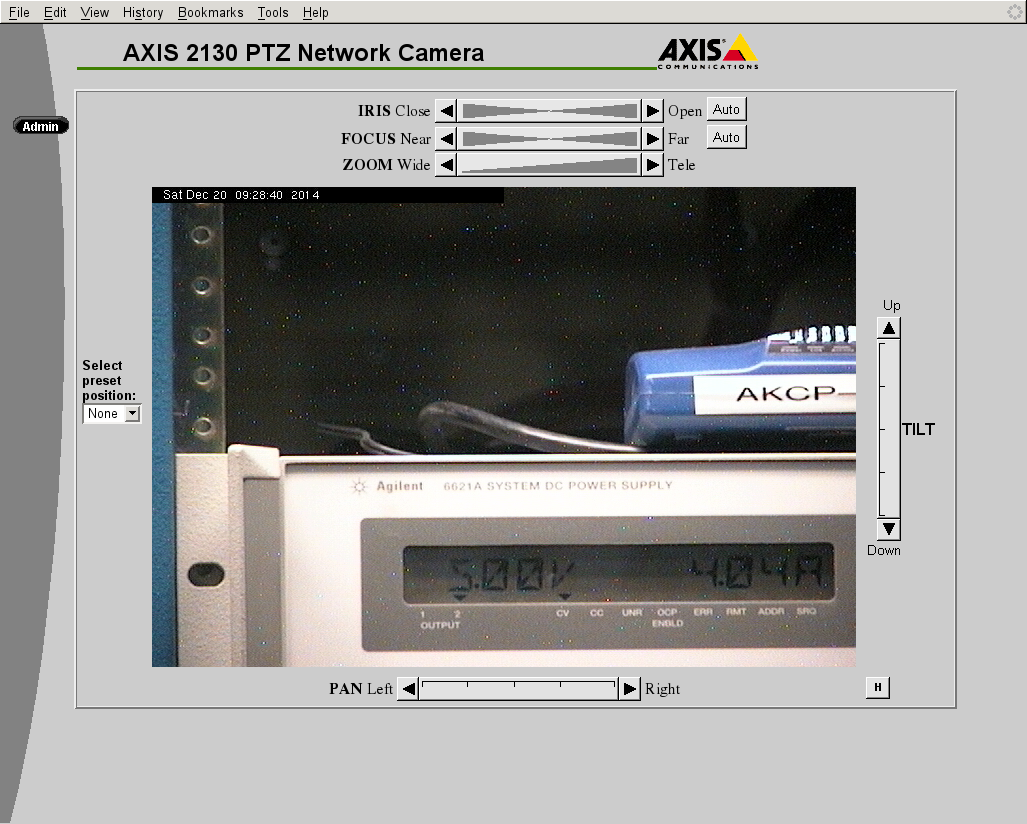
\includegraphics[width=0.5\textwidth]{pics/LVCam_2014_12_20.png}
\caption{\small \label{LVCam} View of the LV screen by webcam (\texttt{cctv11.jlab.org}).}
\end{figure}

      \subsection{Turning ON/OFF High Voltages}

      The high voltage supply of the ECal is controlled and monitored using the EPICS application (see figure~\ref{HV}).  It is accessible via the main EPICS window (\texttt{HV->ECal}), and has buttons to ramp up and down the entire calorimeter's high voltages, and open windows for individual channel control (figure~\ref{HVControl}).

\begin{figure}[htbp]
\center
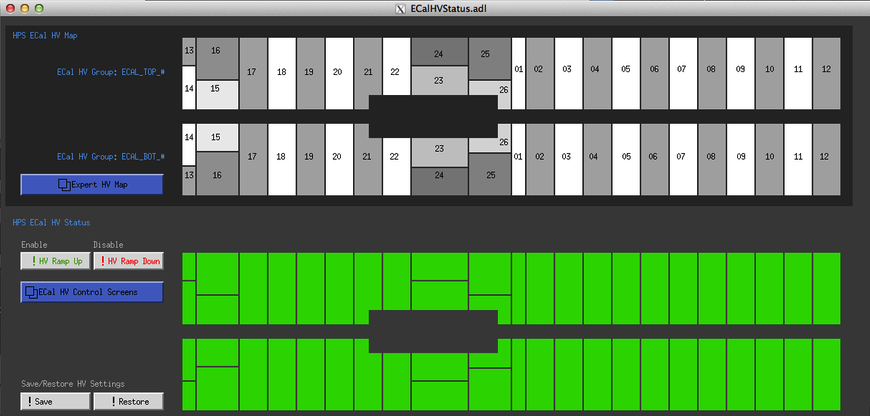
\includegraphics[width=0.95\textwidth]{pics/ecalhvmongui.png}
%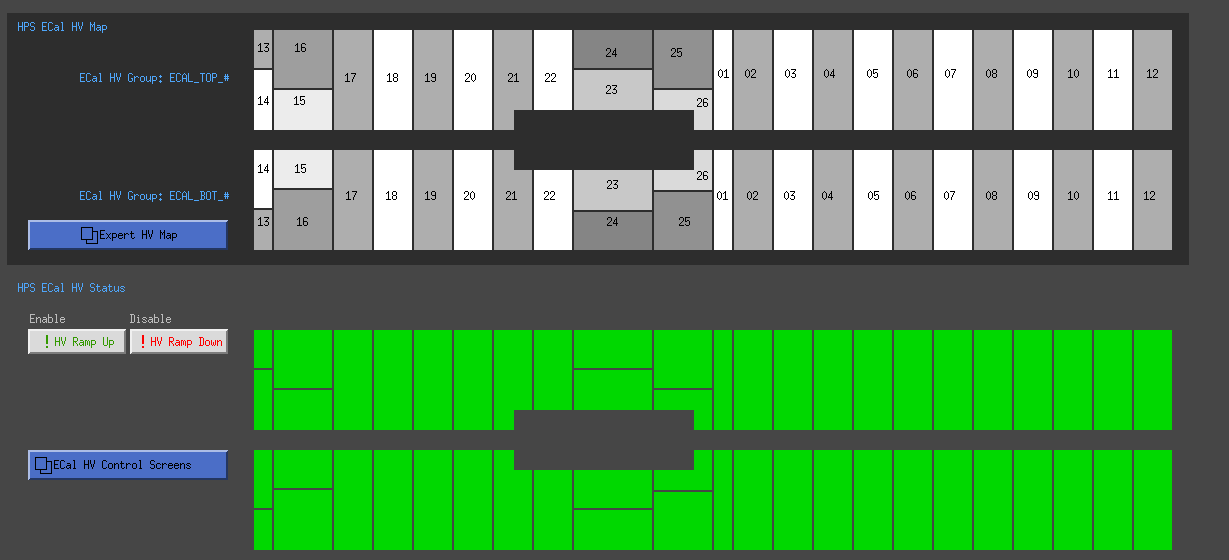
\includegraphics[width=0.95\textwidth]{pics/ecalhv_2014_12_15_16:02:54.png}
\caption{\small \label{HV} View of the EPICS ECal HV monitoring window.}
\end{figure}

   \subsection{HV Current Monitoring}
   Individual channels' currents can be monitoring in figure~\ref{HVControl}, and strip charts should be open for long term monitoring (accessible from the main EPICS GUI (figure~\ref{EPICSmain}) via the ``Strip-Tool'' button).  An example is shown in figure~\ref{fig:hvcurrentstrips}.  Jumps or drifts in current of more than 1 A should be noted in the logbook.

   \begin{figure}[htbp]\centering
       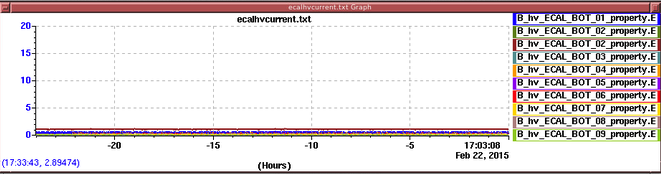
\includegraphics[width=16cm]{pics/hvcurrentstrip.png}
       \caption{HV Current strip charts.\label{fig:hvcurrentstrips}}
   \end{figure}


   \subsection{Responding to HV trips}

      HV problems, in particular trips, are indicated by a red group in the main EPICS GUI (figure~\ref{HV}). Record all HV trips in the log book with indication of the group and run number concerned. HV can be turned back on in the EPICS HV control screen (figure~\ref{HVControl}) accessed in the main EPICS GUI. N.B. The HV can take up to 3 minutes to turn back on so you should end the current run and begin a new one when the high voltage is back on. If you cannot get a HV group to work contact the ECal expert on call.

      {\bf If you encounter more than two HV trips during your shift for the same group, you should notify the ECal Expert.}

\begin{figure}[htbp]
\center
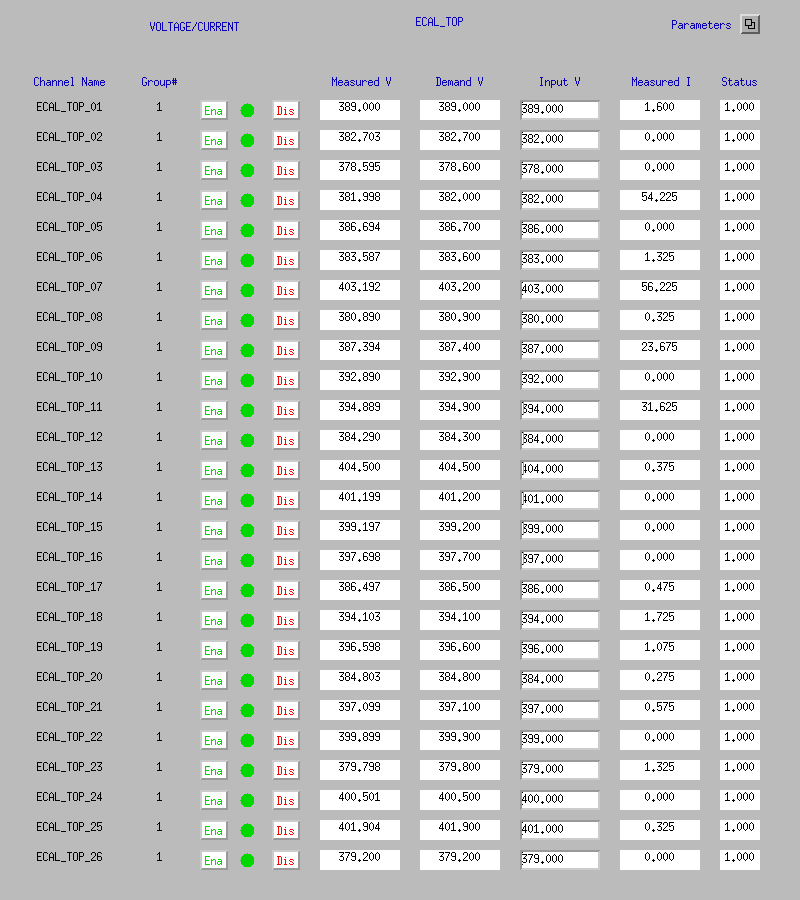
\includegraphics[width=0.85\textwidth]{pics/ecalhv_setting_2014_12_15.png}
\caption{\small \label{HVControl} View of the EPICS ECal HV control window for individual channels.}
\end{figure}

  \section{Strip Charts}
      The most import quantities to monitor with strip charts are temperature and HV current.  There are two programs to view strip charts of ECal EPICS variables.  The older StripTool shown in figure~\ref{temp2} can be found in the HPS\_EPICS gui.  The newer MyaViewer (which adds the ability to retrieve archive information), must be run locally on one of the computers in the counting room (\texttt{clonpcN}, where \texttt{N} is one of the numbers from 11 to 19).  The scripts to run it are in {\it hpsrun}'s path: \texttt{mya\_ecal\_all.sh}, \texttt{mya\_ecal\_temp.sh}, \ldots

   \section{LED Monitoring}

      \subsection{System operations}
      
      The LED system is operated through an EPICS GUI accessible from the main HPS EPICS menu, through Devices, then Flasher (see Figure \ref{FlasherMEDM}).

Shift takers are requested to operate the system in ``Sequence mode'' only. To do so, when requested, click on ``Initialize Flasher'', then verify the TOP frequency is 8000 Hz, and if necessary adjust it trough the proper drop-down menu. Finally, to start the sequence, click on ``Start Blue Seq'' (to use blue LEDs) or ``Start Red Seq'' (to use red LEDs). During such a run the DSC scaler screen allows to check the proper functioning of the channels (figure~\ref{LEDScalers}). 

\begin{figure}[htbp]
\center
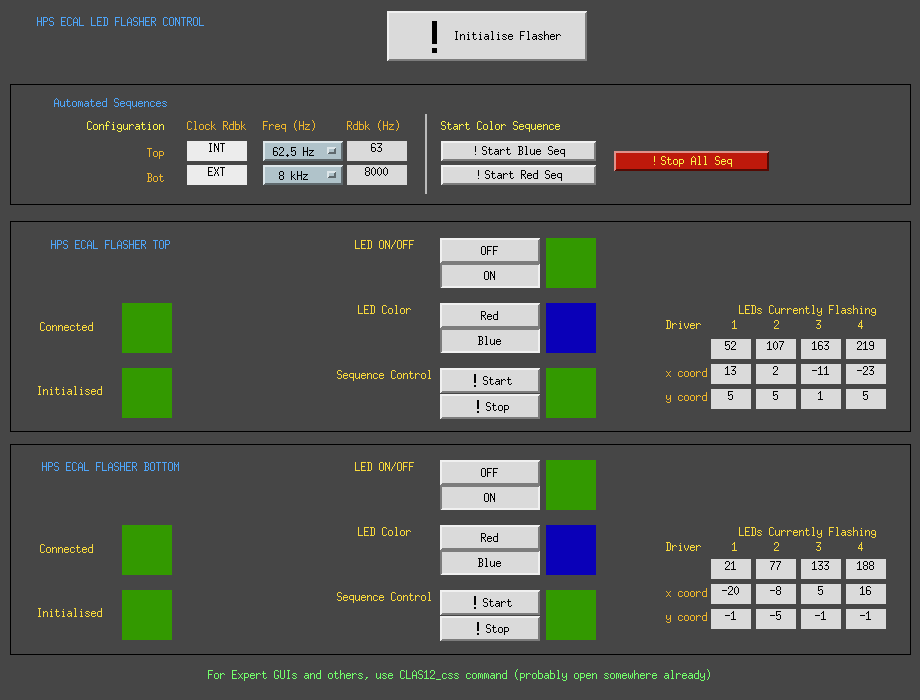
\includegraphics[width=0.75\textwidth]{pics/FlasherMEDM.png}
\caption{\small \label{FlasherMEDM} The HPS-ECAL Led monitoring system EPICS GUI.}
\end{figure}
\begin{figure}[htbp]
\center
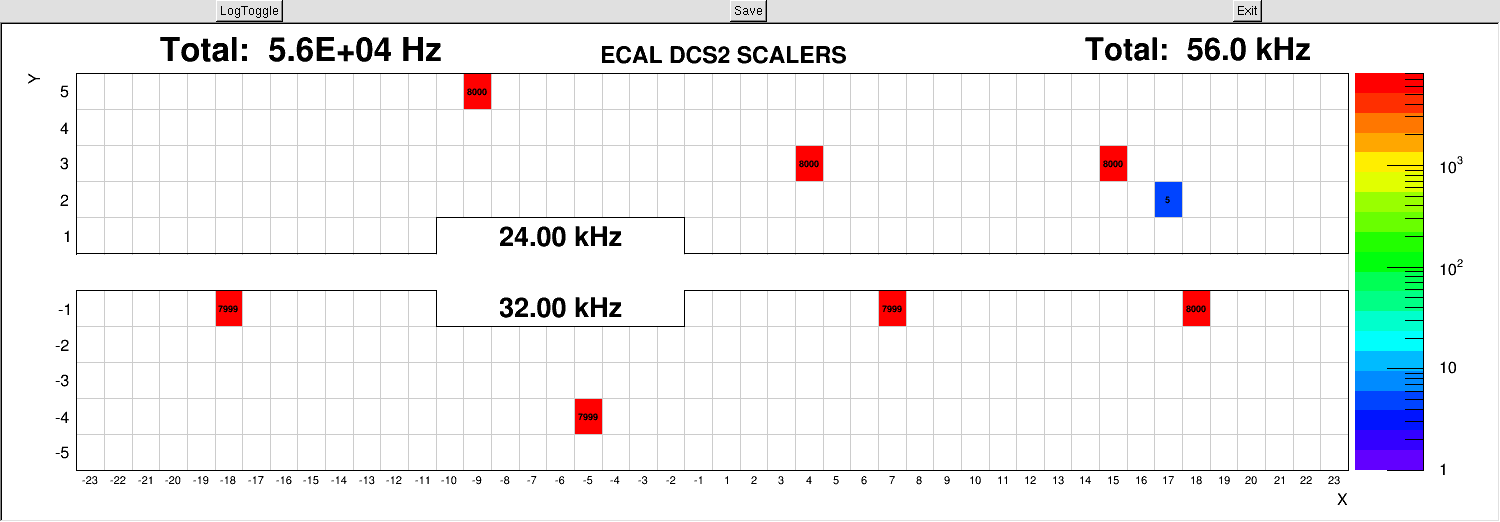
\includegraphics[width=0.95\textwidth]{pics/DSCScalersLED_2014_12_20.png}
\caption{\small \label{LEDScalers} The HPS DSC scaler during a LED run.}
\end{figure}
\newpage
\subsection{Automatic LED Monitoring}
A monitoring app is setup to record all channels successfully registered during an LED run.  It should be started before the LED sequence is started and viewed afterwards, with the command: \begin{center}\$HOME/hps\_software/scripts/startECalLEDSequenceMonitoring.csh\end{center} Make sure to use the hpsrun account before using this command.
  
  {\bf\it ? TODO: Make pedestal viewer app accessible from EPICS gui, and make it save ped files to an absolute path.}

    
\subsection{Taking an LED sequence run}
The following instructions must be followed to take an LED sequence run. This involves setting the DAQ, starting the LED sequence run, and configure the hps-java monitoring app to monitor the data. At the end of the run, the user can upload the relevant information to the hps conditions database, as well as post a log-entry to the HallB electronic logbook.

\subsubsection{Setup}
Follow these instructions to setup the system before takin the LED sequence run.

\begin{description}
\item[Start the DAQ system: ]{Use the run-control to CONFIGURE the DAQ with the proper setting file. Click on ``DOWNLOAD'', then on ``PRESTART''. Wait until the ``GO'' button appears, but {\bf do not click on it yet.}
\bf\it ? TODO: Describe this better: which file to use?
 }
\item[Start the monitoring app: ]{Use the command outlined in the previous section to start the monitoring app.\textcolor{red}{Do this after the run-control shows the ``GO'' button.} When the main gui window shows up, click on the ``Connect button''. The Ecal event display will show up.}
\item[Initialize the LED monitoring sequence:]{In the EPICS gui, click on ``Initialise Flasher'', then on ``!Stop All Seq'' (to ensure there are no previous sequences running). For both controllers, ensure the LED ON/OFF button is set to OFF (you will turn it ON later).} 
\end{description}
      
\subsubsection{Run start, data taking, and run stop}
To start data taking, FIRST click on the ``GO'' button in the run-control gui. Wait 10~s (until the message ``transiction go succeded'' is displayed in the log window and the ``END'' button displays). Then click on ``Start Blue Seq'' or ``Start Red Seq'' in the EPICS gui. Default sequence to take is the BLUE one. Take a RED sequence only if the Ecal expert ask you to do so.

While the LED sequence is running, you can look at the monitoring application to check data being recorded. The event display will show 8 crystals at time with a signal. A full sequence will take $\simeq$ 10 minutes to complete.

{\bf  The DAQ system is not set up to end the run when the LED sequence is completed.} 

Therefore, use the EPICS gui to check the sequence status (RED is OFF, GREEN is ON). The user can confirm the sequence has actually ended by looking at the ECal Event display: no crystals are ON at this stage.
When both sequences are OFF, first turn OFF both controllers (LED ON/OFF, click on OFF), then use the DAQ run control to END the run.



\subsubsection{Analysis at the run end}

When the run ends, the monitoring application automatically will recognize this, and the analysis of the measured data will start. 

A pop-up will appear, asking the user if he wants to upload the LED data that has been measured to the HPS conditions database: uploaded quantities are the average channel response to LED pulses and the RMS. Before confirming this, the user is required to have a look at the average charge per LED, displayed in the monitoring app: tab Ecal Led Sequence, sub-tab Sequence Map. The average channel response should be in the range $\simeq 20 \div 30$. 

An automatic log entry in the Hall B logbook will also be made, with the Sequence Map image. The user is requested to complete the comment form with any relevant observation, and then click on ``OK''

{\bf {\it TODO: print a reference map and aks the user to compare with that}}

\subsection{Quick 2-Minute LED Run for Simple Channel Status Check}
This just counts threshold crossings in the discriminators, which is sufficient for checking that all channels are alive with LEDs.  This full test of all 442 channels requires only 2 minutes, requires no changes to the DAQ configuration, and is completetely independent of the hps-java monitoring app.

  \begin{enumerate}
      \item With a quiet detector, execute the command \texttt{runEcalLedTest.sh}.  This will open a gui showing accumulated scaler rates in all 442 ECal channels.  
      \item Start a ``LessFast'' LED sequence.
      \item Check that all channels are uniformly populated after sequence is finished.
  \end{enumerate}

   \section{Making a cosmic calibration run}

   In addition to the calorimeter, the cosmic PMTs should be powered on.  Their HV control is under ``beam'' in the main EPICS gui's HV section.  They are named \texttt{ECal\_cosm1} and \texttt{ECal\_cosm2}.  The DAQ configuration should be set to \begin{center}\texttt{hps\_cosmic\_mode1\_thresh0.cfg}\end{center}  It takes at least one full day of data to acquire sufficient statistics for a cosmic calibration.

   \section{Taking a Pedestal Run}

   Pedestals are calculated at running luminosity with DAQ configuration \begin{center}\texttt{hps\_ecal\_pedestal\_mode7\_thresh50.cfg}\end{center} and monitored and analyzed with HPS's hps-java monitoring app via the command:
   \begin{center}\$HOME/scripts/ECalCalculatePedestals.sh\end{center}
Once the user deems the statistics sufficient in the monitoring plots, the app should be disconnected from the ET-ring and then output will be files \texttt{fadc37.ped} and \texttt{fadc39.ped} in the current working directory.  An expert should place them in the proper location for the DAQ to read.

{\bf\it ? TODO: Make pedestal viewer app accessible from EPICS gui, and make it save ped files to an absolute path.}

      \section{Scalers}

         Rates seen by the ECal are available in the EPICS (Fig \ref{Scalers}), they represent the rates as seen from the FADC and TDC electronics. The difference is mainly due to their different thresholds. One can also see scalers from the DAQ GUI (figure~\ref{DAQscalers}), this indicates the rates of clusters reconstructed by the trigger electronics. These numbers should all remain constant within ~10\% during stable beam operation. A strong increase is the indication of bad beam conditions or is due to the presence of a new source of noise, in the latter case, please contact ECal expert on call.

\begin{figure}[hbp]
\center
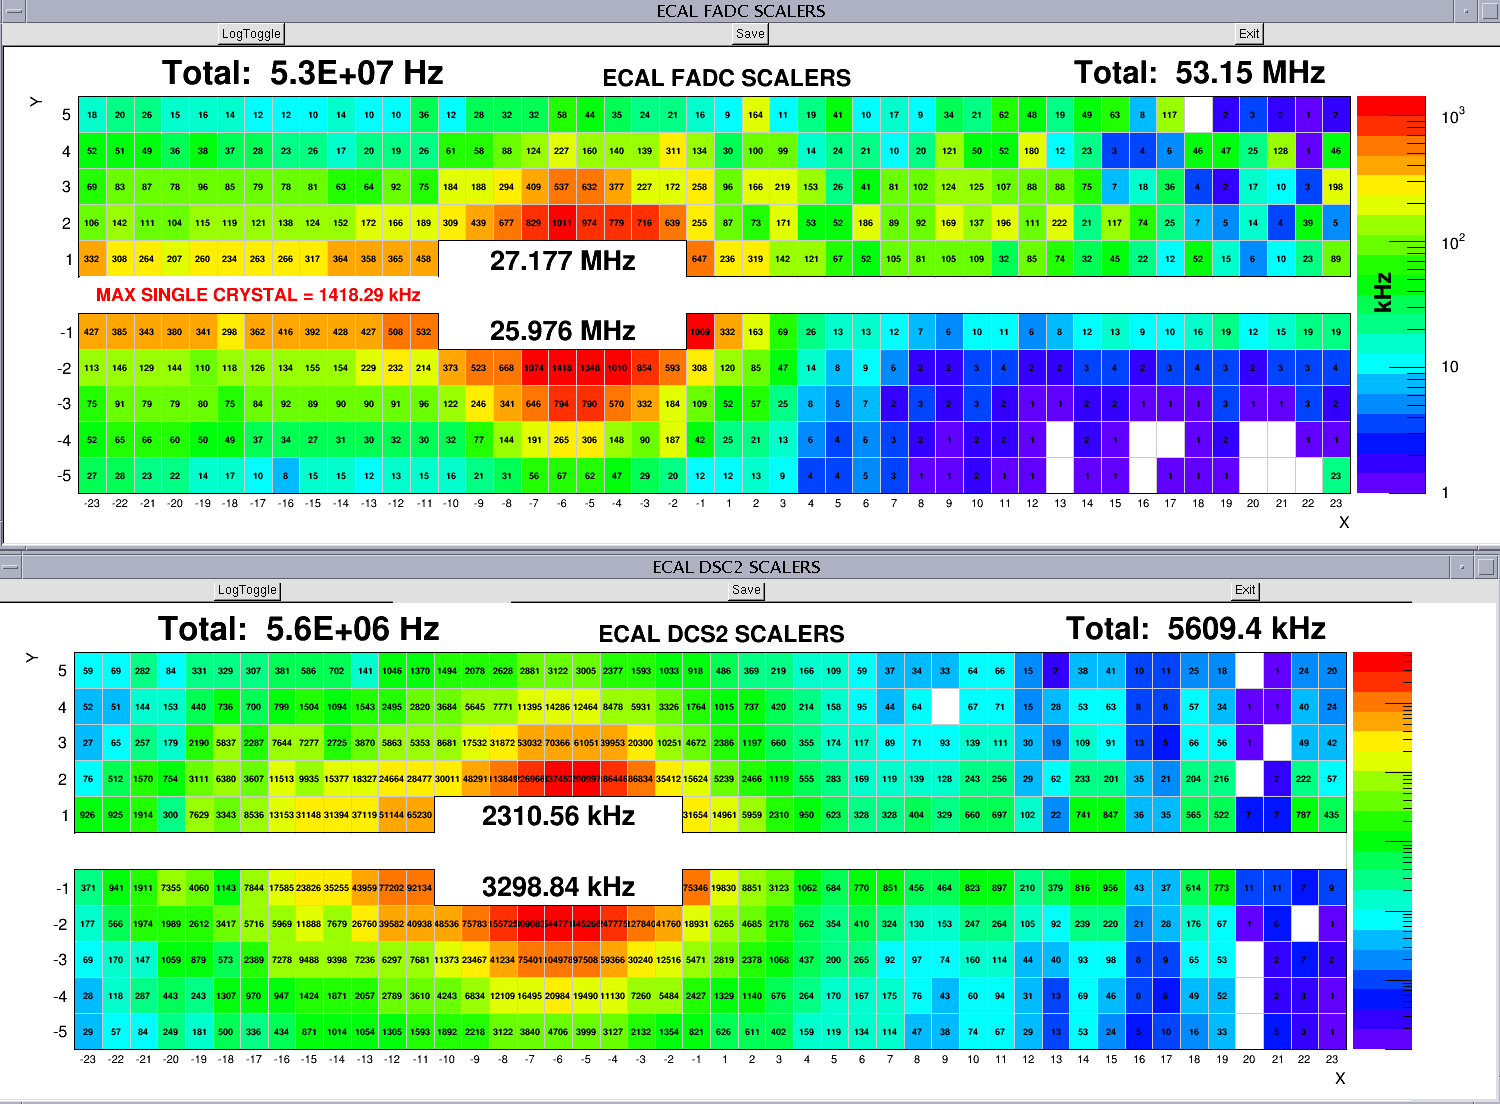
\includegraphics[width=0.75\textwidth]{pics/ECAL_FADC_SCALER_2014_12_20.png}
\caption{\small \label{Scalers} View of the EPICS FADC and DSC2 scalers window.}
\end{figure}

\begin{figure}[hbp]
\center
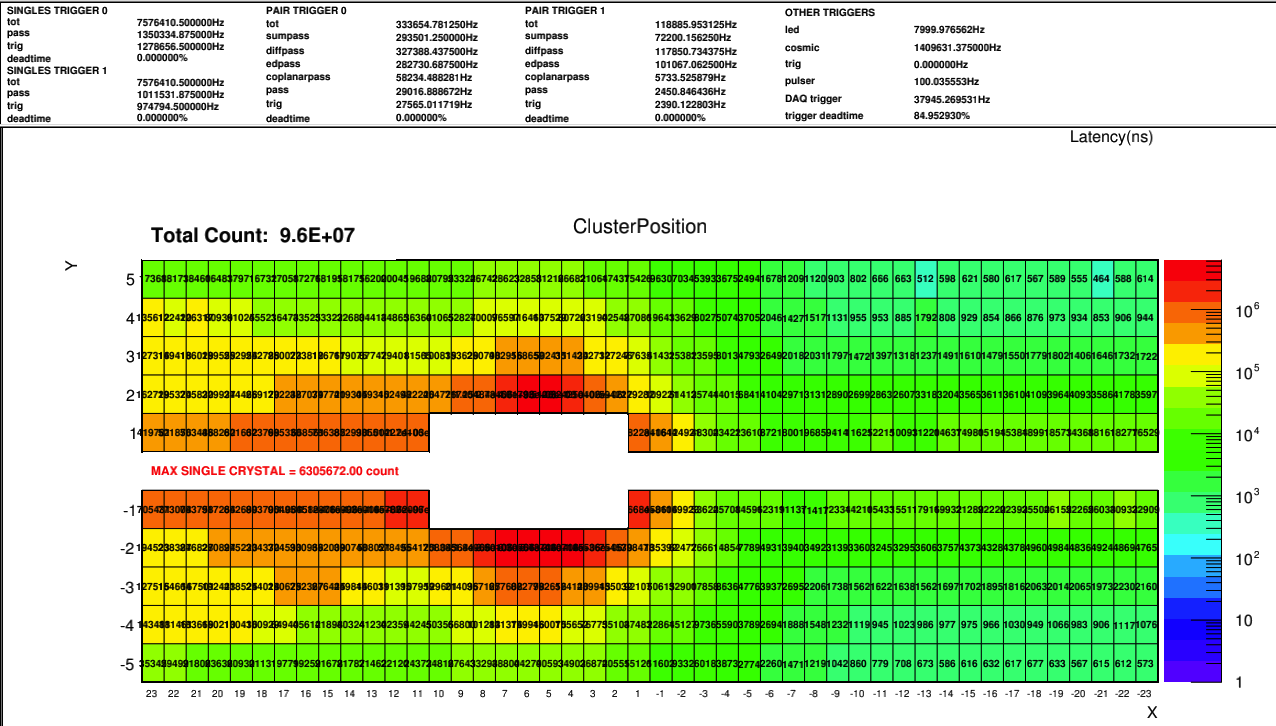
\includegraphics[width=0.75\textwidth]{pics/ecal-cluster-12-20-14.png}
\caption{\small \label{DAQscalers} View of the DAQ scaler window.}
\end{figure}

\newpage

\part{ECal Experts Resources}

   \section{Localization of ECal elements for experts}

{\bf REMINDER:} Since the ECal is within 3 feet of the beam line it needs to be surveyed by RADCON before any work can be done on it.
   {\footnotesize
\begin{itemize}
\item
The chiller is located beam-left just downstream of the calorimeter on the ground.
\item
The LED controllers are located at the top of the rack closest to the beamline in the Alcove.
\item
The TDC crates are in the rack closest to the beamline in the Alcove.
\item
The FADC crates and calorimeter signal splitters occupy the rack furthest from the beamline in the Alcove.
\item
    The HV supply is on the Pie Tower in the rack closest to the beamline.  See figure~\ref{fig:HVPHOTO}.
\item
    The LV supply is on the Pie Tower at the top of the middle rack. See figure~\ref{fig:LVPHOTO}.
\end{itemize}

\begin{figure}[htbp]\centering
    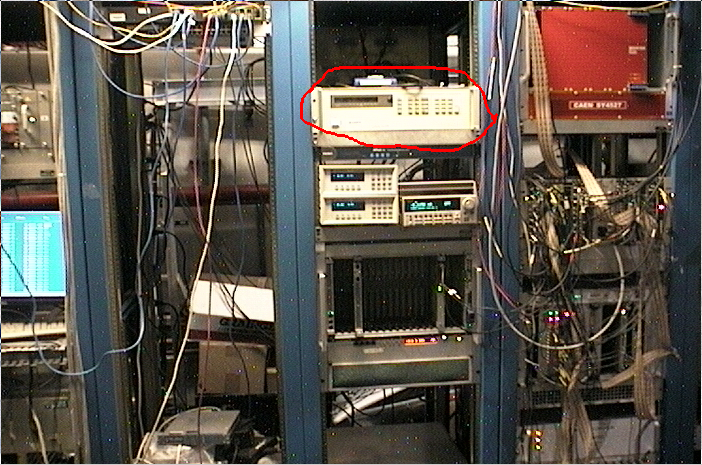
\includegraphics[width=7cm]{pics/ECALLVPHOTO2.png}
    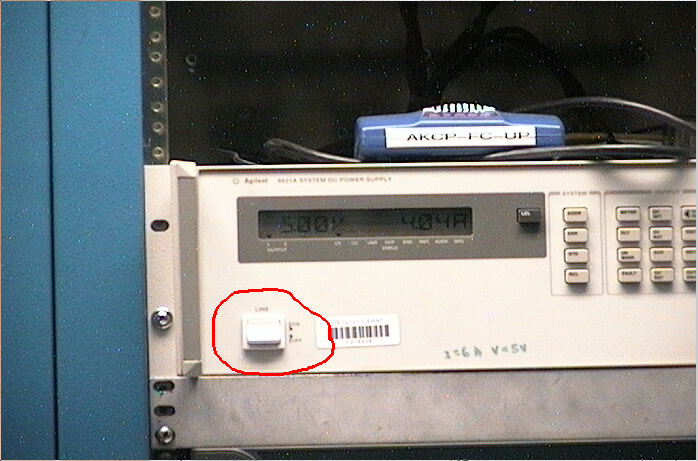
\includegraphics[width=7cm]{pics/ECALLVPHOTO.png}
    \caption{Location of Agilent LV power supply near the top of the middle rack in the pie tower.  Power switch circled.\label{fig:LVPHOTO}}
\end{figure}
\begin{figure}[htbp]\centering
    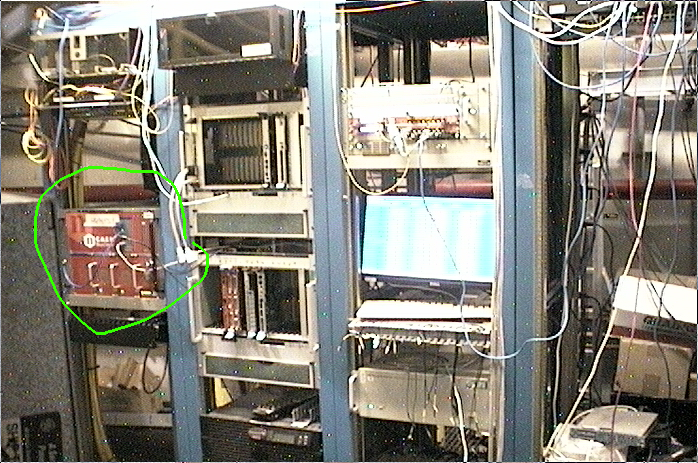
\includegraphics[width=10cm]{pics/ECALHVPHOTO.png}
    \caption{Location of the CAEN SY1527 HV power supply in the left-most rack in the pie tower.  Key for on/off is in the lower right corner of the crate.  It is labeled ``HVHPS1''. \label{fig:HVPHOTO}}
\end{figure}

   \section{Cooling system}

   The cooling system is using a Thermo Scientific chiller that can be controlled through EPICS (\ref{ChillerCam}). The setting should not be modified; the temperature setting should be fixed at 17 degrees Celsius. In case of problem with the chiller contact ??? (who can take care of these in Hall-B engineer group?).  The manual for the chiller can be found here:

   {\noindent\footnotesize\url{http://www.nist.gov/ncnr/upload/Circulating-Bath\_Thermo-Scientific\_NESLAB-RTE-7.pdf}}
     \subsection{Rebooting the Chiller After Power Failure}
     If the chiller loses power while in local mode, the ``power'' button must be pressed manually to restart it after power is restored.  In case it loses power while in remote mode, a procedure is necessary to reset it after power is restored:
   {\footnotesize
     \begin{enumerate}
         \item Hold the ``up'' and ``down'' arrow buttons simultaneously for 10 seconds.
         \item Press the ``computer'' button to go into local mode.
         \item Press the ``power'' button to turn it off.
         \item Press the ``power'' button to turn it on.
         \item Press the ``computer'' button to return to remote mode.
    \end{enumerate}
    }

    \subsection{Restarting the Chiller IOC}
    Chiller IOC runs in ``procserv'', a wrapper that automatically runs and restarts services and provides access to them via telnet.  To restart the chiller's IOC:
   {\footnotesize
   \begin{enumerate}
       \item \texttt{`ssh hpsrun@clonsl1'}
       \item \texttt{`softioc\_console iocchiller'} and type user's password if necessary.
       \item \texttt{`ctrl-x'} to restart the IOC
       \item \texttt{`ctrl-]'} to quit to telnet
       \item \texttt{`quit'} to exit telnet
   \end{enumerate}
   }

   \subsection{Restarting the Temperature Monitoring IOC}
   Thermocouples are used to monitor the temperature inside and outside the calorimeter.  To restart the IOC that reads these:
   {\footnotesize
   \begin{enumerate}
       \item \texttt{`ssh hpsrun@clonsl1'}
       \item \texttt{`softioc\_console ioctempSens'} and type user's password if necessary.
       \item \texttt{`ctrl-x'} to restart the IOC
       \item \texttt{`ctrl-]'} to quit to telnet
       \item \texttt{`quit'} to exit telnet
   \end{enumerate}
   }



   \section{Changing LV settings}
      Low voltage power supply should be set at $\pm5$V. The low voltage supply might have difficulties to get at this level because of the high current. If that was the case check, with all power supplies off, that all connection are goods. Then contact run coordinator to see if LV power supply addition is possible. 

   \section{High Voltage}
   \subsection{Restarting the HV IOC}
   Occaissonaly the soft IOC for the HV needs to be manually restarted.  Symptoms of this condition include errors messages from EPICS when trying to turn on/off voltages and white blocks in the main HV screen (figure~\ref{HV}).  The IOC always needs to be restarted if the mainframe is power cycled.  
   
   Currently, the HV IOC runs in a ``screen'' on \texttt{clonioc1}.  To restart it, follows these steps:
   {\footnotesize
   \begin{enumerate}
       \item \texttt{`ssh hpsrun@clonioc1'}
       \item \texttt{`screen -ls'} to list running screens
       \item \texttt{`screen -x ECALHVIOC'} to attach to the screen running the IOC
       \item \texttt{`ctrl-c'} to kill the IOC
       \item \texttt{`up-arrow ; return'} to restart the IOC
       \item \texttt{`ctrl-a-d'} to detach from the screen
   \end{enumerate}
   }
   If for some reason this does not work (e.g. no screen named something like \texttt{ECALHVIOC} is listed in \#2, or \#5 does not start the IOC), you can start from scratch:
   {\footnotesize
   \begin{enumerate}
       \item \texttt{`ssh hpsrun@clonioc1'}
       \item \texttt{`screen -S ECALHVIOC'} to create and attach to a new screen named \texttt{ECALHVIOC}
       \item \texttt{`cd /home/nerses/github\_test/epics/apps/iocBoot/iocECal\_Voltages'}
       \item \texttt{`./st.cmd'} to start the IOC
       \item \texttt{`ctrl-a-d'} to detach from the screen
   \end{enumerate}
   }
   Don't leave a terminal open connected to this screen.
   \subsection{Changing HV Settings}
      {\bf NOTE:} Changing voltage settings should be taken care of in coordination with the ECal group (contact R.~Dupre). Current setting can be increased in case of need, please document this change in the log book and notify the ECal expert on call.

 {\bf NOTE:} The ECal HV groups had to be renumbered in the EPICS, the correspondence map (figure~\ref{ExpertMap}) is available in the main ECal HV monitoring window with the Expert HV Map button.

\begin{figure}[htbp]
\center
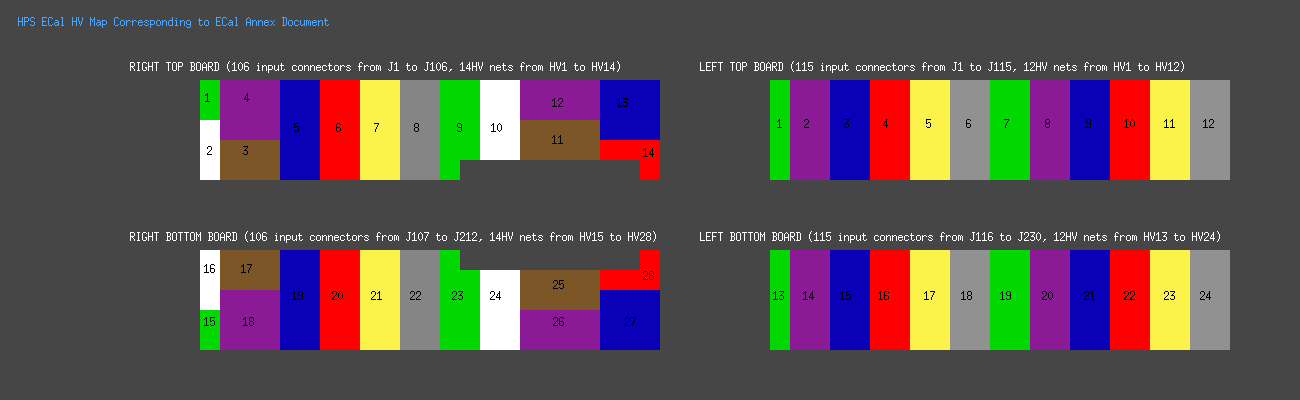
\includegraphics[width=0.95\textwidth]{pics/ecalhv_expertmap_2014_12_15.png}
\caption{\small \label{ExpertMap} Expert HV channel map for reference.}
\end{figure}

      If for some reason some channels were to drop in gain (or increase) or if the current drawn increases in a group, it might be necessary to change the HV settings in the expert ECal EPICS control (Fig.~\ref{EHV}). A modification of the voltage will lead to a modification of the gain used by the trigger system, these values need to be updated at the same time!
      \subsection{HV Save/Restore}
      A system to save and restore the entire calorimeter's voltage settings is available via buttons in the main monitoring window.  If the voltage setpoints are changed, a backup should be made of the new settings.  This must be run as a user in group \texttt{clas-4};  user \texttt{hpsrun} does not have sufficient priveleges to save/restore voltage settings. 
      An example of the restore window is shown in figure~\ref{fig:hvrestore}

\begin{figure}[htbp]
\center
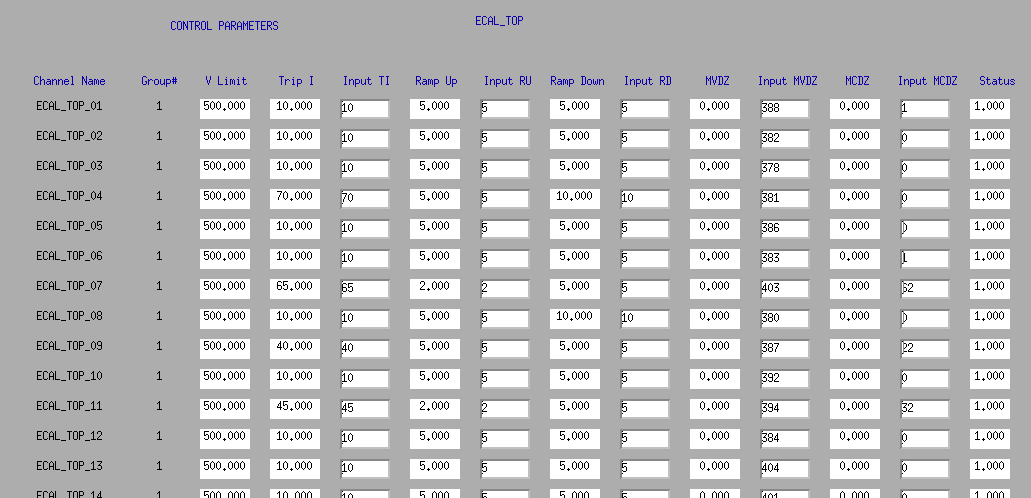
\includegraphics[width=0.85\textwidth]{pics/ecalhv_parameters_2014_12_15.png}
\caption{\small \label{EHV} View of the EPICS HV expert control window. It is accessed from the parameters button in the ECal HV control screen \ref{HVControl}}
\end{figure}

\begin{figure}[htbp]\centering
    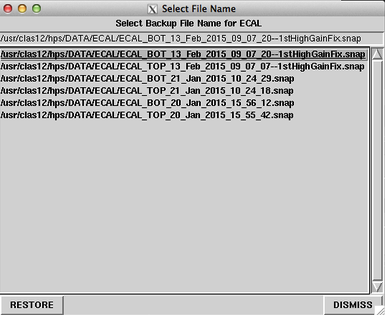
\includegraphics[width=8cm]{pics/hvrestore.png}
    \caption{The gui interface to save/restore HV settings.  \label{fig:hvrestore}}
\end{figure}

   \subsection{Long Term HV monitoring}

   An hourly snapshot of HV currents is stored by a cron job (and in the EPICs and MYA databases).  Currently the easiest way to view it is as user \texttt{hpsrun} on \texttt{clonpcNN} by excuting the command:
   \begin{center}
   \texttt{\$HOME/.ecalhv/plotEcalHV.py}
   \end{center}
The product should be a plot like figure~\ref{HVhistory}.

\begin{figure}[htbp]
\center
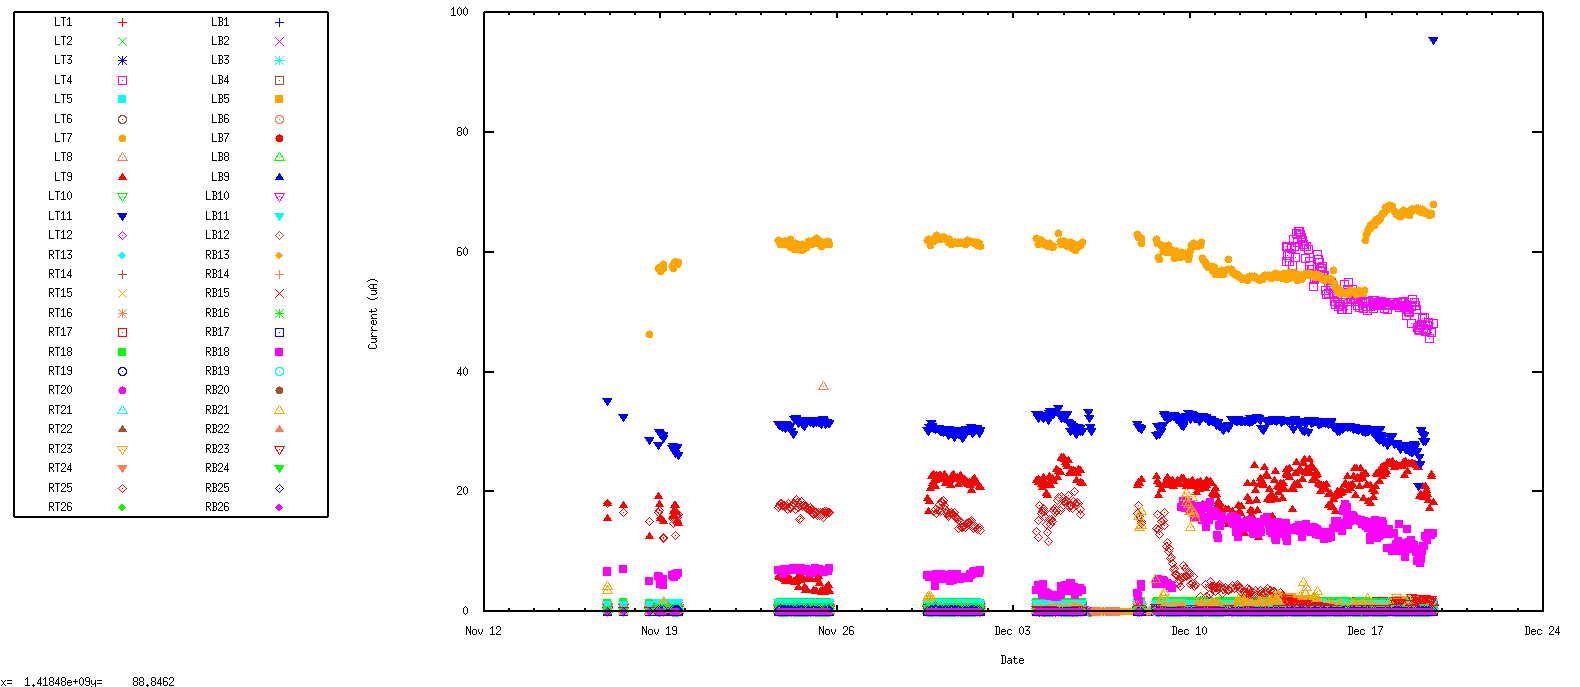
\includegraphics[width=0.95\textwidth]{pics/ECALHVCURRENTS_2014_12_20.png}
\caption{\small \label{HVhistory} Expert HV current history.}
\end{figure}

   \section{Disconnection of a Channel and Preamplifier Replacement}
     
      In last resort, to recover a HV group that is tripping one can disconnect the faulty channel causing trouble. To do so, you need to find exactly which channel is involved! It might be obvious from data, if the channel was already very noisy, else you will have to test the channels of the group one by one. This is a lengthy operation and should only be attempted with the authorization of the run coordinator and in coordination with the ECal Group. It necessitates that the Hall-B crew moves the ECal out of the beam line and to open it.

   \section{LED system for experts}

This section has to be replaced with instructions to use the CLAS\_css GUI.

\begin{figure}[htbp]
\center
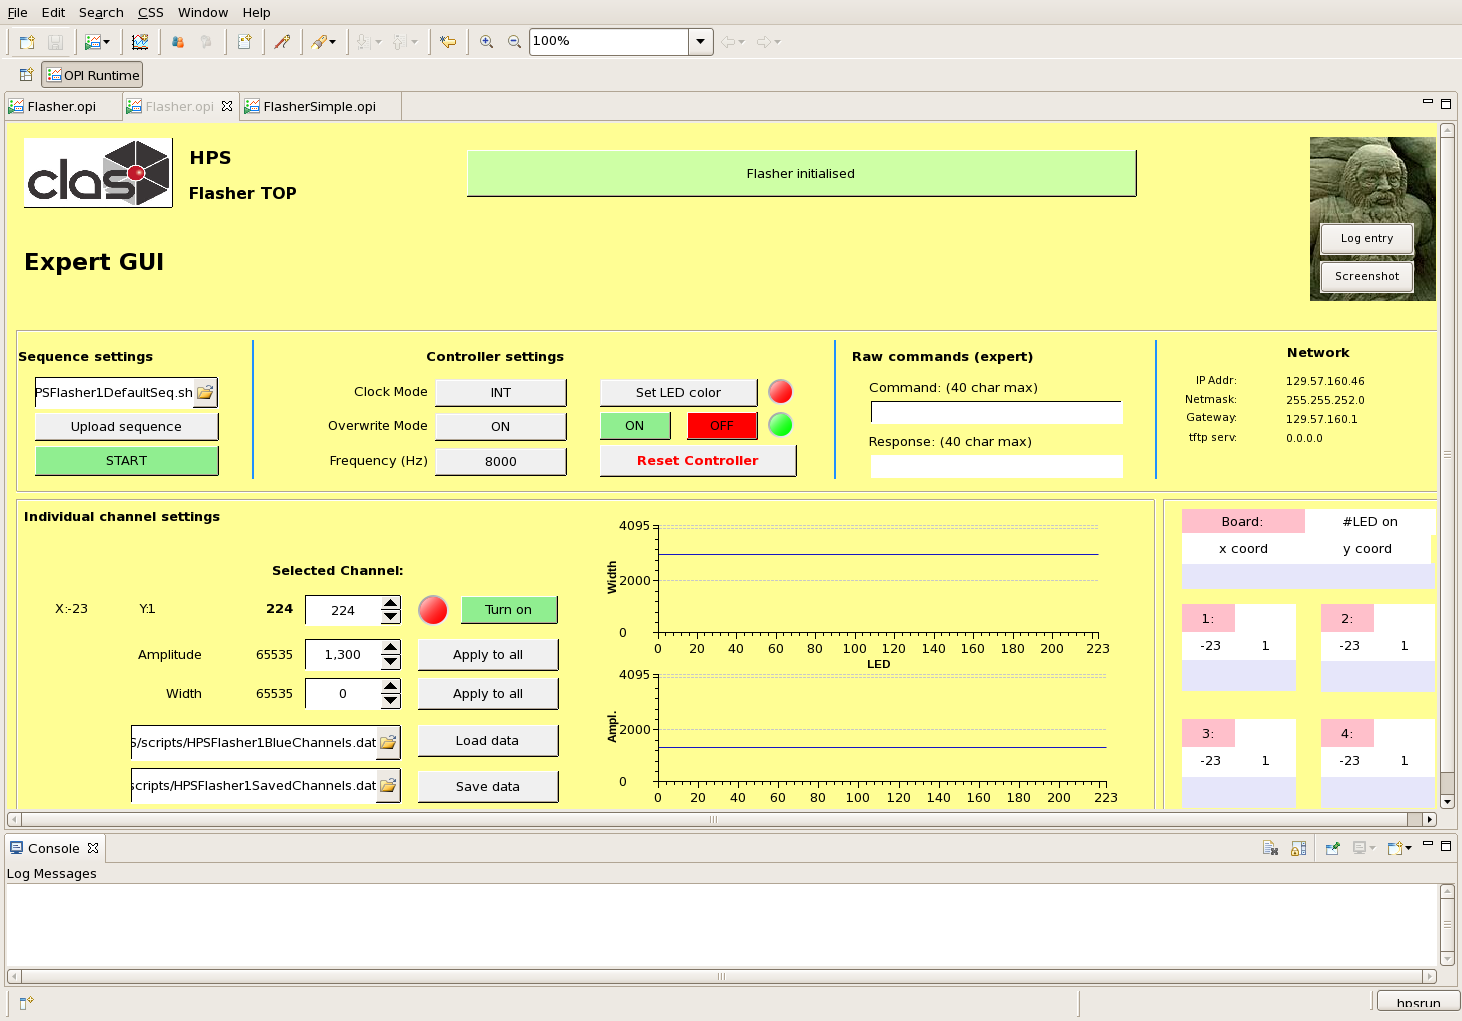
\includegraphics[width=0.85\textwidth]{pics/LEDExpert_2014_12_20.png}
\caption{\small \label{LEDexpert} View of the LED expert controls.}
\end{figure}

\end{document}
